\chapter{System Implementation, Testing and Validation}
\section{Introduction}
This chapter describes how the Students’ results handler was implemented. The implementation was driven by the desire to achieve the objectives set at the beginning of the project.

\section{System Implementation}
This section contains an overview of the project implementation; it highlights the major components and the operation of the system as well as the different user interfaces and activities that allow users to interact with the system.

\subsection{Implementation tools}
This application has various faces that can be accessed by the student, the Administrative Assistant, the Academic registrar and a potential employer. Various tools are used to develop these for example, the truffle framework which provides an environment to write smart contracts in solidity and compile them. Other tools include Ganache which is a blockchain network simulator on a local machine.\\~\\
The front end of the application is developed in languages such as JavaScript, HTML and using the bootstrap framework as well.

\subsection{User Interface Design}
The system can be accessed through a web application on a browser of choice. However, the browser should be able to support the MetaMask file extension. This is helpful in enabling the user access the blockchain network.

\subsubsection{Account Creation}
For a student still on normal academic progress, he/she has the ability to register and have an account. This requires the student id number and a password. \\~\\
However, for access to the blockchain, the student or any other user intending to access the verified transcript has to create an account on the Ethereum network. During this process, a seed phrase is automatically generated for a user and he/she only has to create a password.

\begin{figure}[!h]
\center
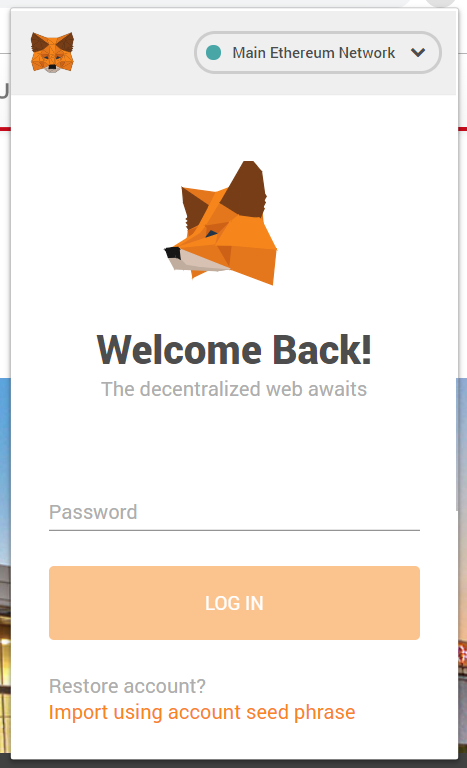
\includegraphics[scale=0.6]{images/metamasklogin.png}
\caption{Loging into the ethereum network}
\end{figure}

\subsubsection{Results}
\textbf{Viewing Results}\\~\\
This page can be accessed by a logged in student or an administrative assistant. The student can only view his/her results whereas the administrative assistant can view the results of various students.
\textbf{Manipulating results}\\~\\
In addtion to viewing results of various students, the adminsstrative assistant can also add/edit students’ results.
